Based on the analysis, as one of the most advanced documentation generator is Swagger UI, it will be my main inspiration.
Also, the Swagger UI is a well-known tool in the software development community, and it is used by many companies and projects.
The Swagger UI works in a way that the website is a static website by default and the endpoints, types, and more are defined in a definition file.
This file is a OpenAPI YAML or JSON file, which is then parsed and displayed on the website~\cite{swagger-ui-definition-file}.
I think this is a good approach, as it separates the data from the view.
Thanks to this, the data can be easily changed and the website will regenerate dynamically in the browser.
The deployment of the website is also easier, as it is just a static website, which can be hosted on any web server, and updating the definitions can be part of different deployment process.

First, I will try to analyze, if I could use Swagger UI directly, or if I need to create my own website.


\section{Swagger UI for gRPC}

% TODO: OpenAPI, swagger UI extensions


As gRPC has its specifics, and it is not based the same way as OpenAPI, I will need to create my own website.


\section{gRPC Reflection Possibility}
% Issue with comments in Reflection, reflection feasability
% Discuss the options and possibilitions


\section{gRPC-Web limitations}
% gRPC-Web limitations, and how it affects the design
% Possibility of full gRPC server implementation in the future, but also may-be not necessary if gRPC-Web supports it
% grpc-web-text and grpc-application content types


\section{Architecture}
The architecture of the website will be based on the Swagger UI, but it will be adjusted to the gRPC specifics.
The website will be a static website, which will take a gRPC definition file for showing all gRPC related parts.
The gRPC definition file from the proto files or gRPC reflection and its format will be most probably either JSON or YAML\@.
These formats are common in software development, and they are also used by the Swagger UI, which I take the inspiration from.

I have created a diagram of the architecture of the website, which is shown in the figure~\ref{fig:grpcflair-architecture}.
There are two places where the generation of the common format starts.
The first one is from the .proto, the second one is from the gRPC reflection.
Both methods will generate the same format, which will be then used by the website.
The website will be a static website, which will be generated from the common format on the fly using JavaScript.
The user of the website will be able to see all the methods, types, and enums, which are defined in the gRPC definition file.
They will also be able to call the methods and see the responses in the website.
When they invoke the request, the website will select the correct backend (gRPC-Web or other implementation) and it will the server.
The server then returns the response, which is then displayed in the website (the responses can be shown gradually as for example the server streams responses).

% The overall process description - state diagram - (with the help of the diagram I have)
% Swagger UI JSON inspiration

\begin{figure}[hbt!]
    \centering
    \captionsetup{justification=centering}
    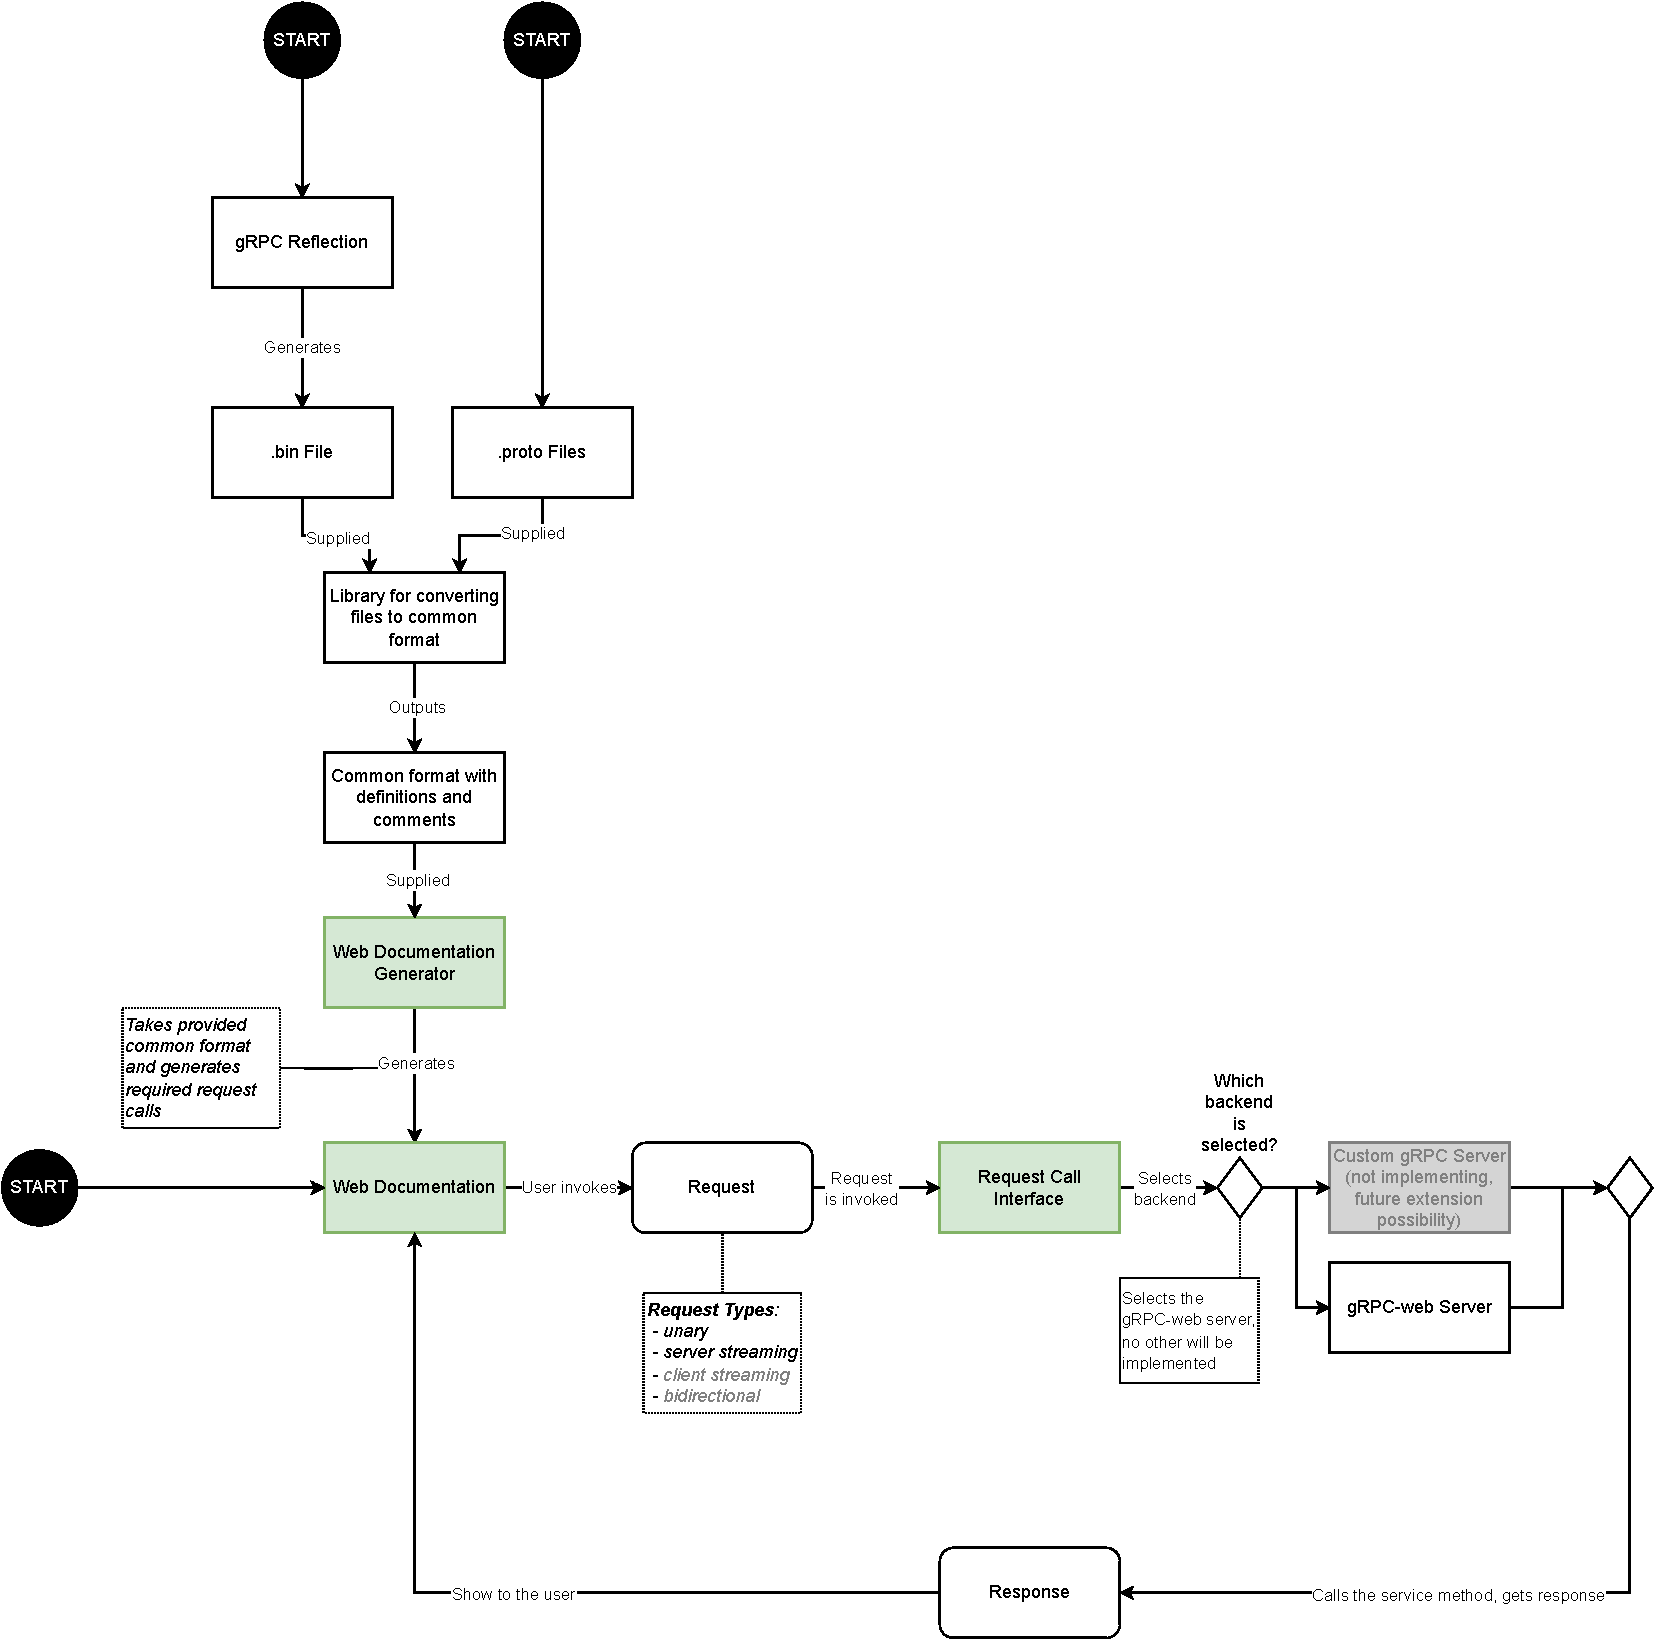
\includegraphics[width=1.0\textwidth]{images/design/grpcdoc-architecture}
    \caption{Architecture}
    \label{fig:grpcflair-architecture}
\end{figure}


\section{Common Format}

\subsection{OpenAPI}
% Why not use OpenAPI -> It's made for REST, not gRPC, I would have to map it -> already existing solutions

\subsection{grpc-protoc-gen-doc}

\subsection{gnostic}

\subsection{proto3-json-serializer}

\subsection{protobufjs}
% Protobufjs, protobufjs-cli

\subsection{Summary}
% Why not use my own parsing


\section{Website Design}

\subsection{Proto Files Generator}

\subsection{gRPC Reflection Generator}
% Discuss the options and possibilitions

\subsection{Website Wireframe}
% Inspiration and main focus
% Section: Main Page
\ref{fig:wireframe-main-layout}

\begin{figure}[hbt!]
    \centering
    \captionsetup{justification=centering}
    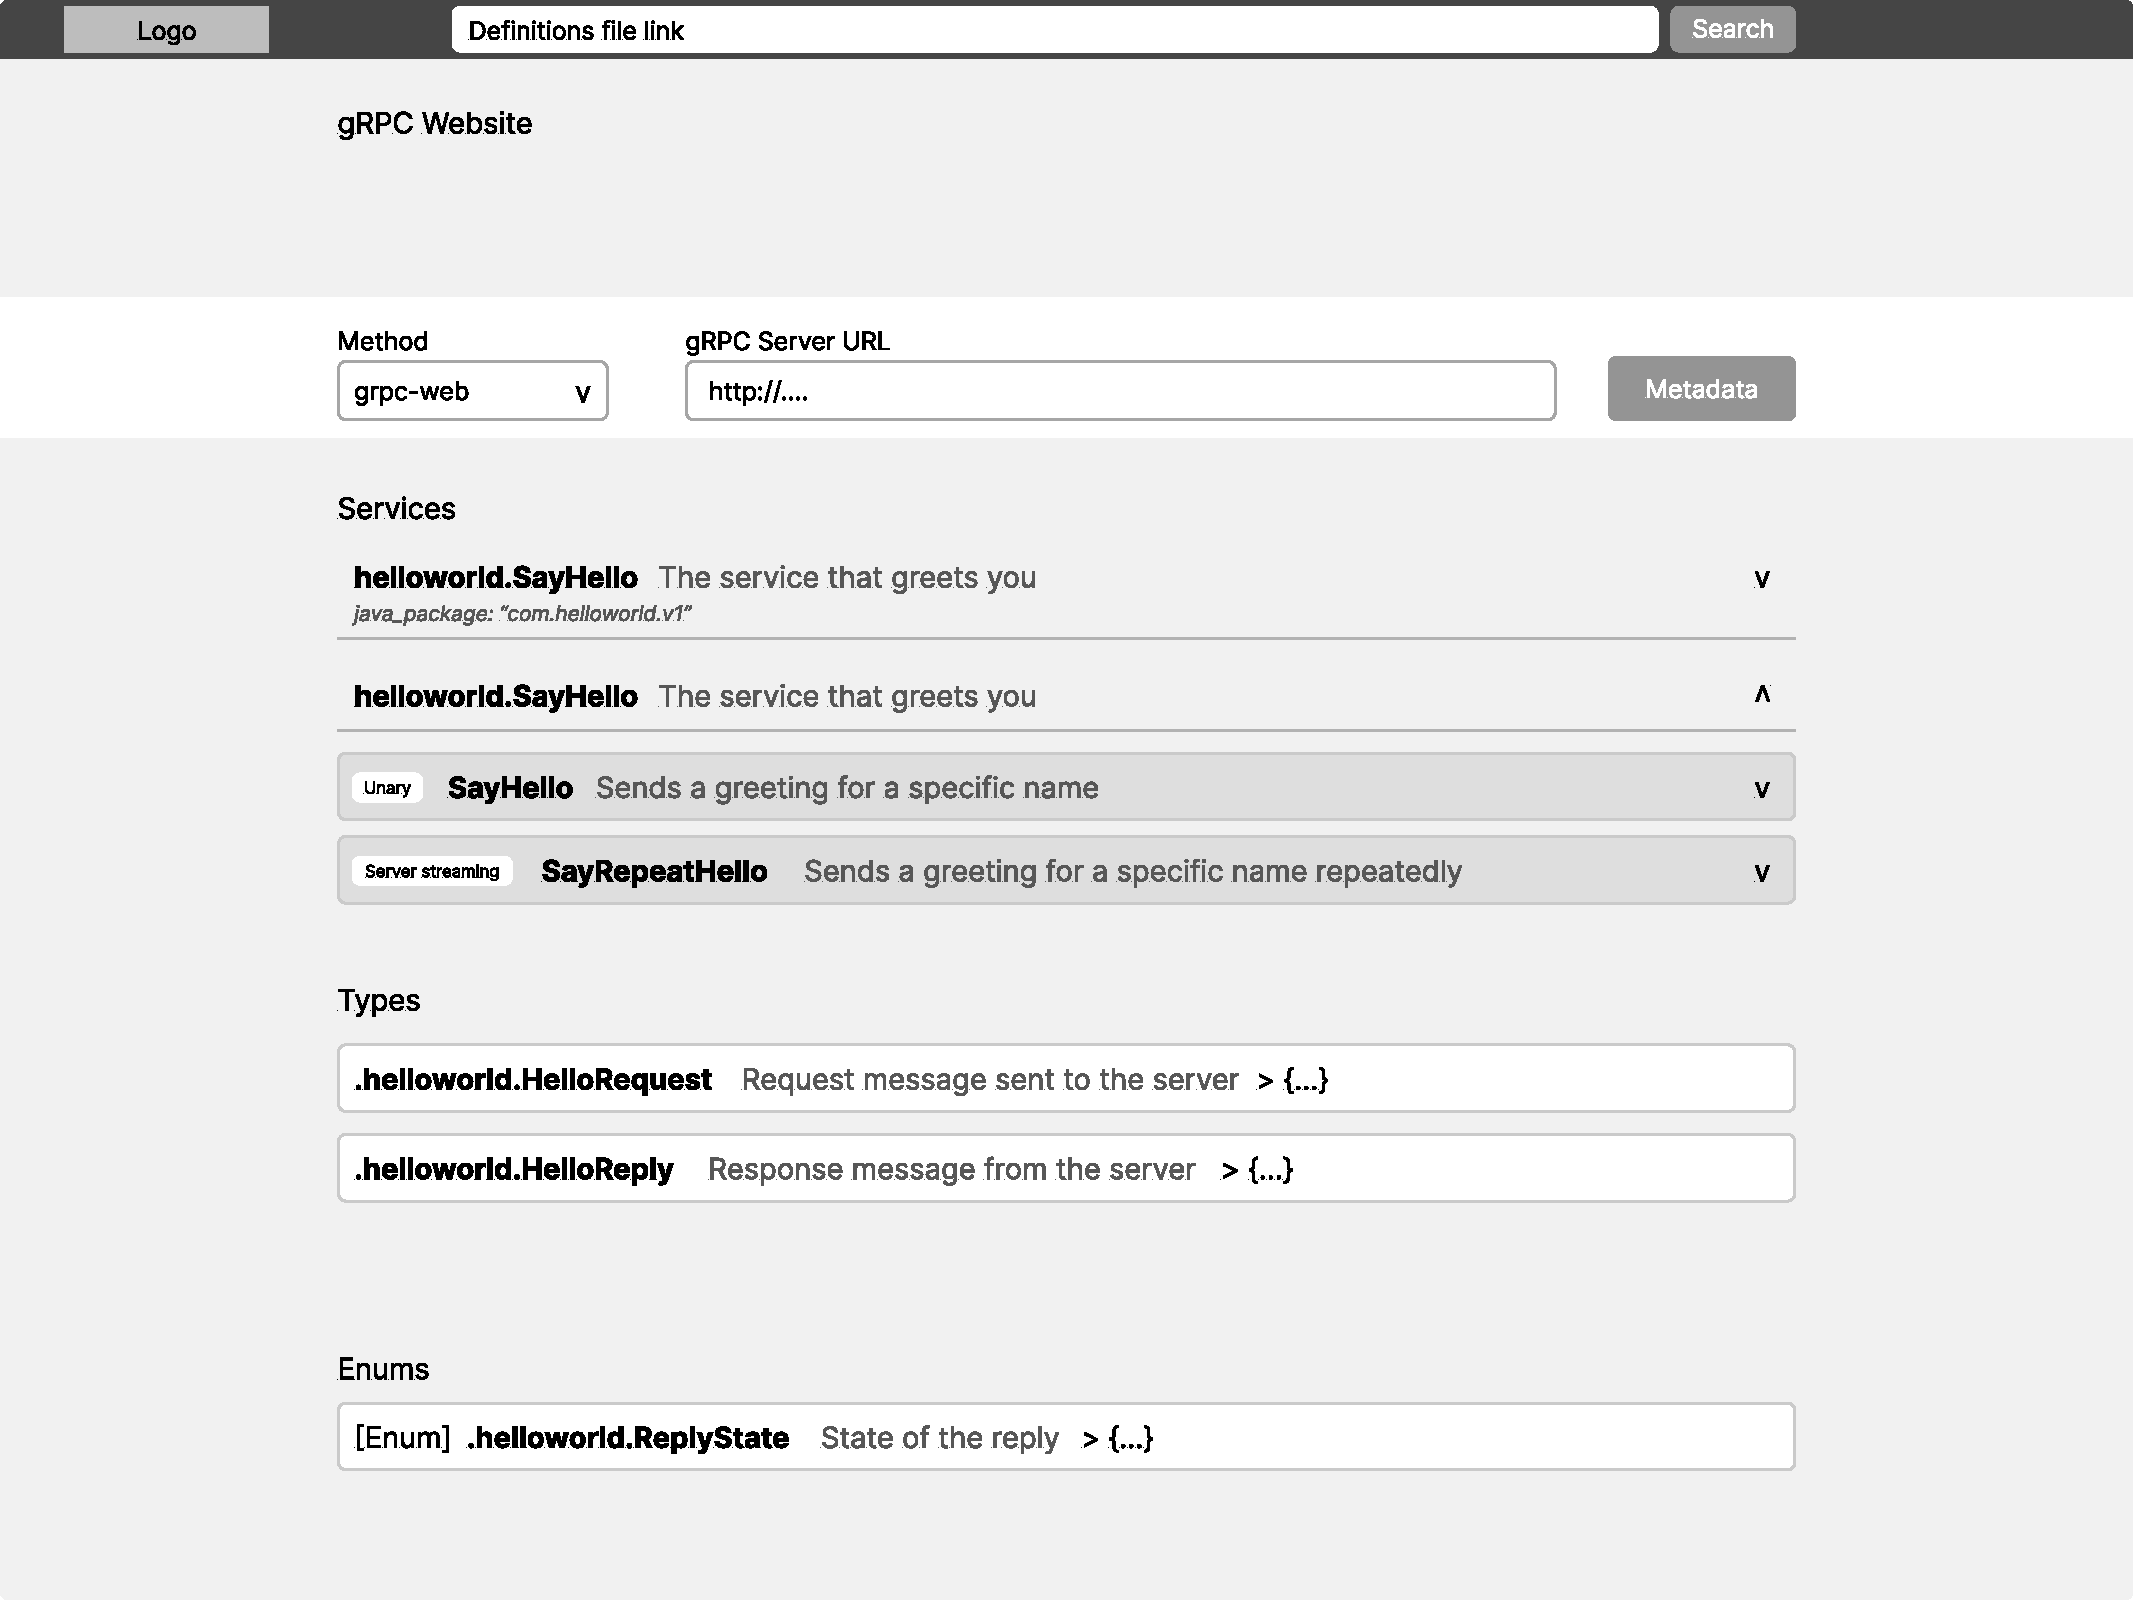
\includegraphics[width=1.0\textwidth]{images/design/wireframes/main-layout}
    \caption{Main Layout Wireframe}
    \label{fig:wireframe-main-layout}
\end{figure}

\subsubsection{Method Wireframe}
% Section: Method, and it's detail with forms, JSON, etc
\ref{fig:wireframe-method}

\begin{figure}[hbt!]
    \centering
    \captionsetup{justification=centering}
    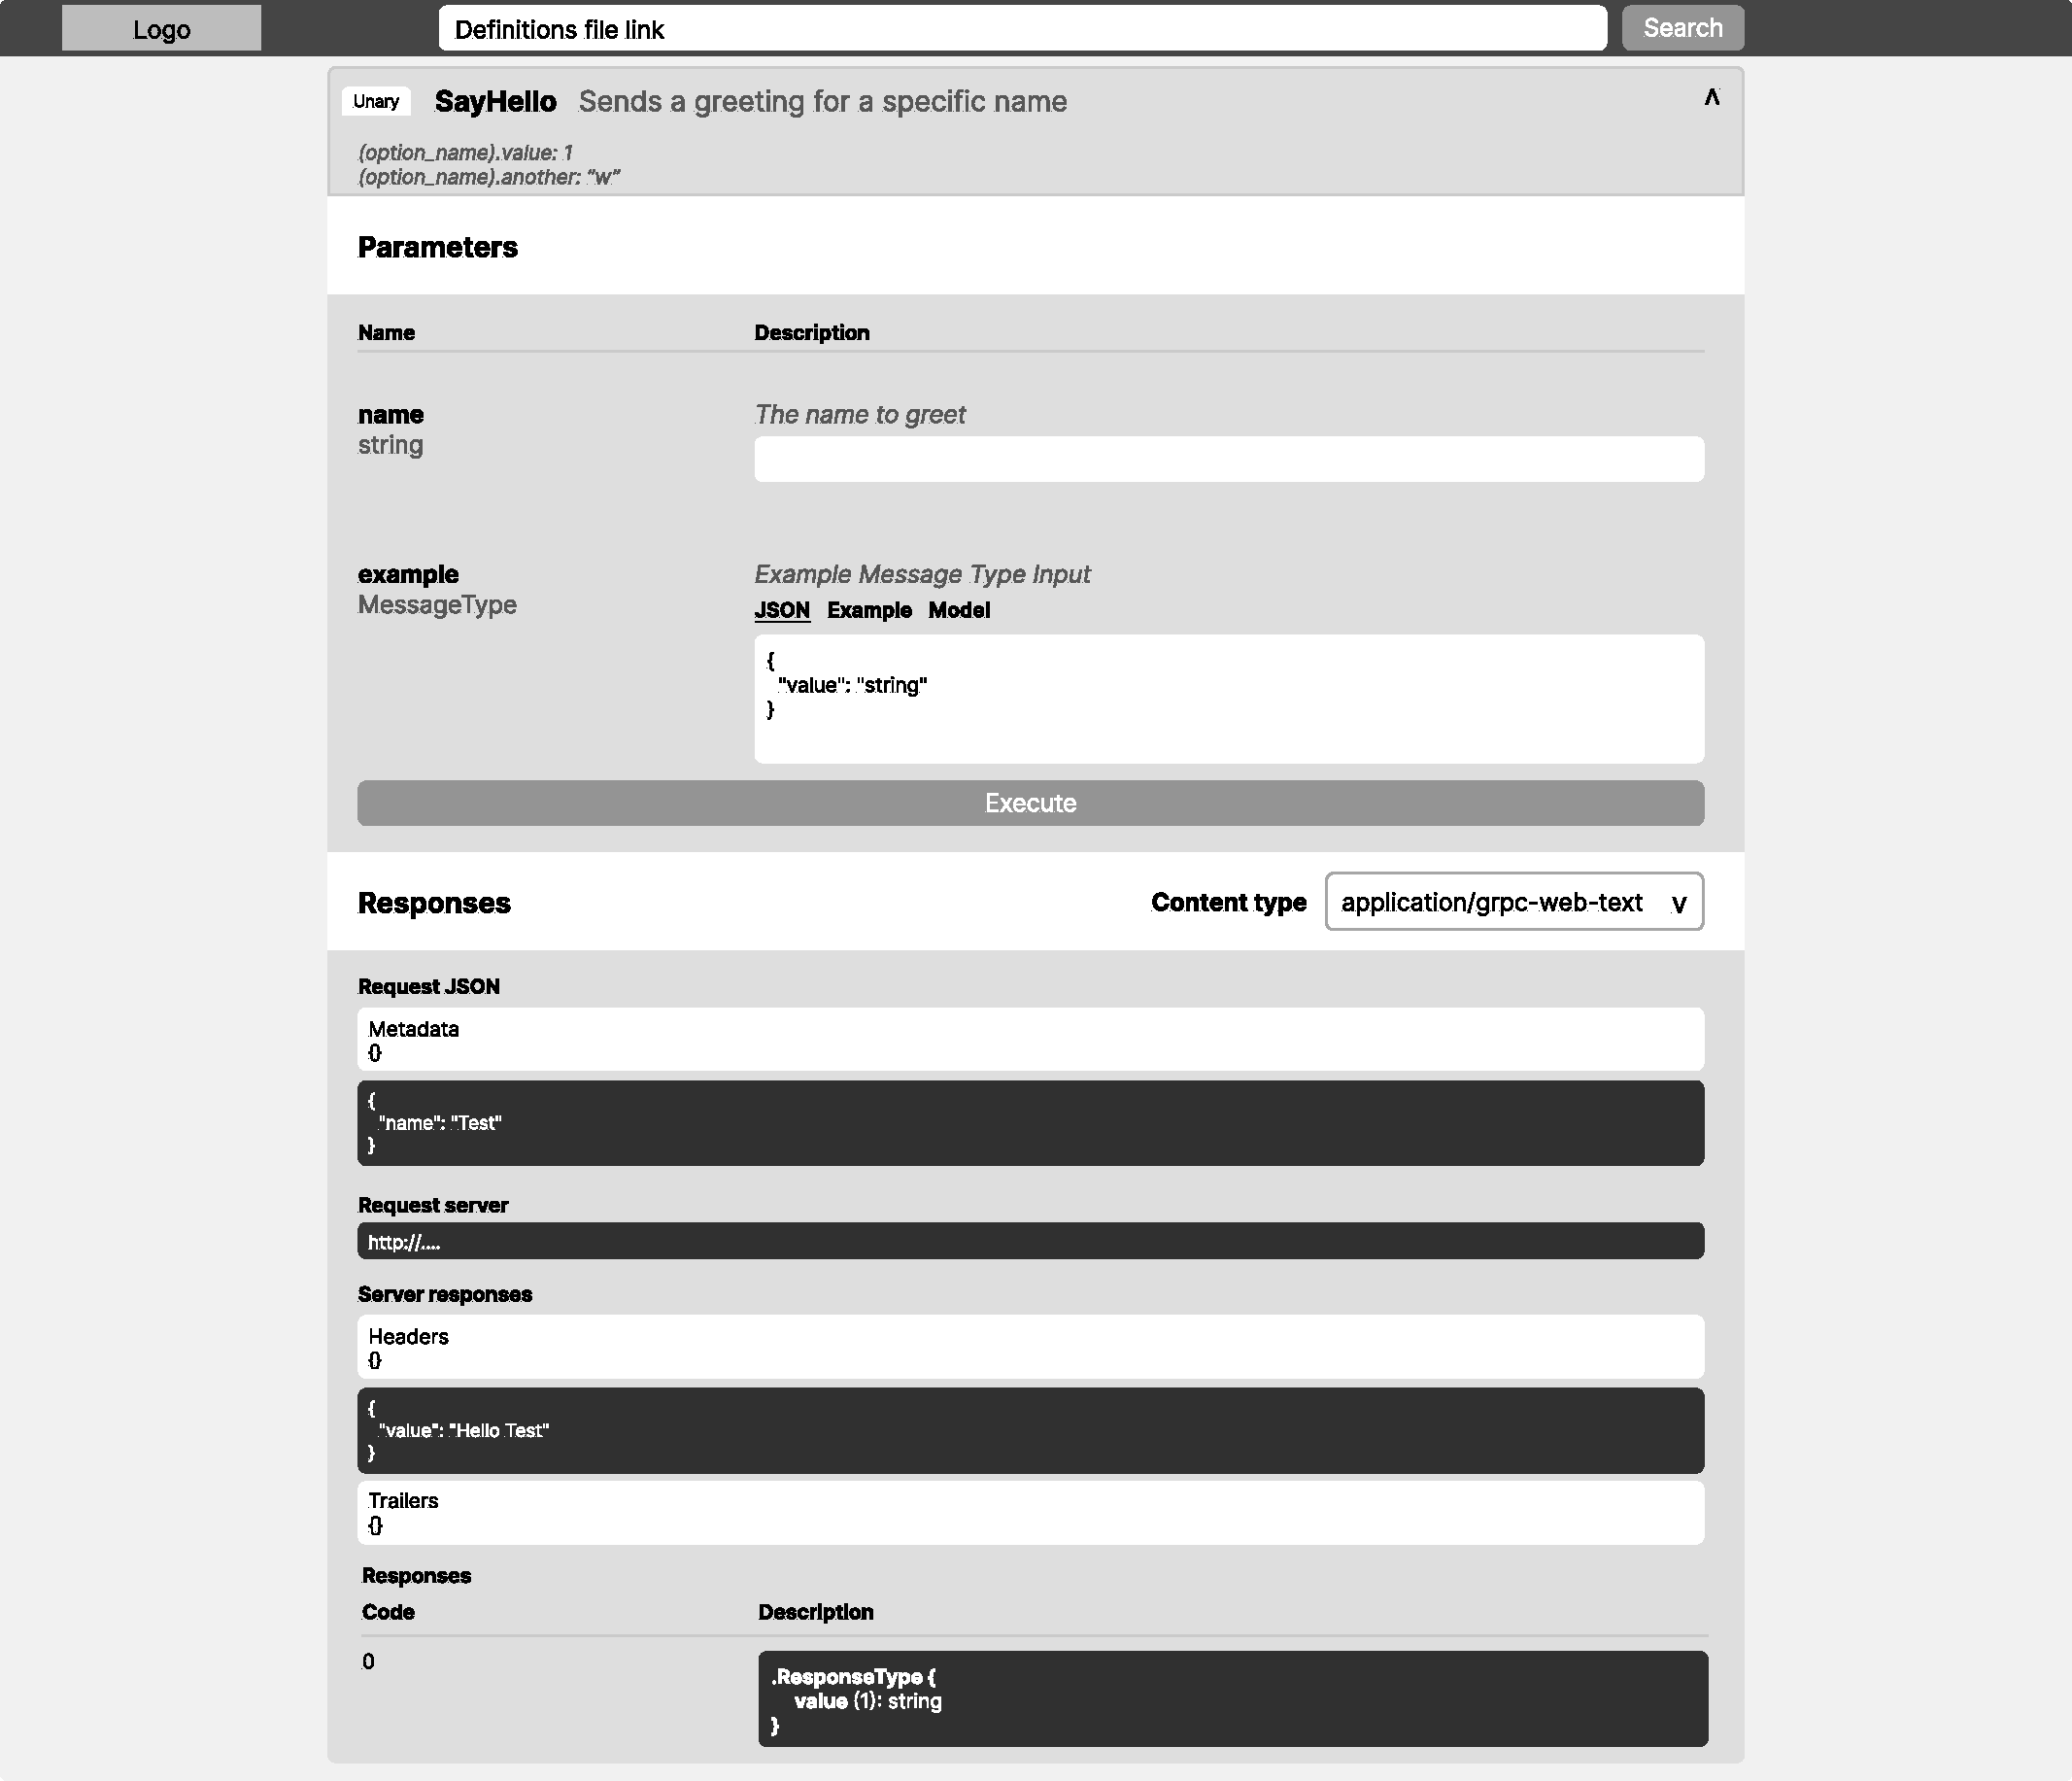
\includegraphics[width=1.0\textwidth]{images/design/wireframes/method}
    \caption{Method Wireframe}
    \label{fig:wireframe-method}
\end{figure}

\subsubsection{Type and Enum Wireframe}
% Section: Type & Enum
\ref{fig:wireframe-type}
\ref{fig:wireframe-enum}

\begin{figure}[hbt!]
    \centering
    \captionsetup{justification=centering}
    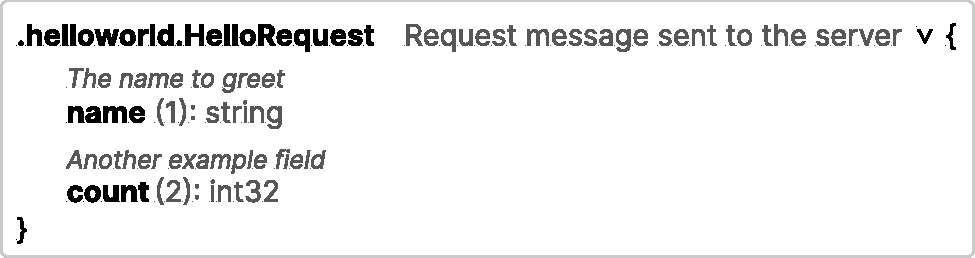
\includegraphics[width=0.8\textwidth]{images/design/wireframes/type}
    \caption{Type Wireframe}
    \label{fig:wireframe-type}
\end{figure}

\begin{figure}[hbt!]
    \centering
    \captionsetup{justification=centering}
    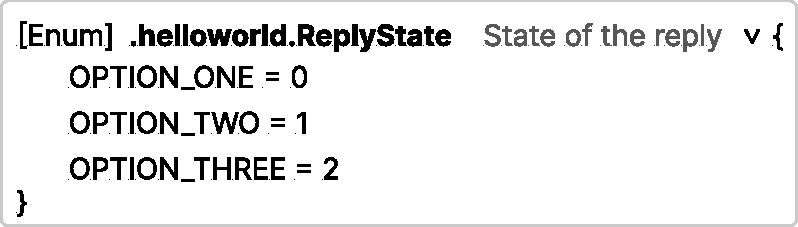
\includegraphics[width=0.8\textwidth]{images/design/wireframes/enum}
    \caption{Enum Wireframe}
    \label{fig:wireframe-enum}
\end{figure}


\section{Fulfillment of Requirements}
%Samotné grafické rozhraní aplikace splňuje požadavek N1.
%Zobrazení dialogového okna s informacemi pro inicializaci obrazu softwaru Syllabus Plus splňuje požadavek F1.
%Uspořádání dat do sloupců a rozdělení obrazovky na dvě části splňuje požadavek F16.
%Libovolný výběr dat a částečné převody u všech pohledů splňuje požadavky F2, F3, F5, F6, F9, F10 a částečný export u pohledu časových lístků splňuje požadavky F17 a F18.
%Požadavek F4 je splněn pouhým přidáním sloupce navíc k pohledu místností, není nutné cokoli v návrhu měnit, jedná se pouze o implementaci.
%Požadavek F7 je implementačně závislý, nesouvisí s návrhem rozhraní.
%Možnost výběru informací u převodu časových lístků pokrývá požadavek F8.
%Tlačítko pro spárovaní položek splňuje požadavek F11.
%Dialogové okno před převodem dat do systému Syllabus Plus splňuje požadavek F12 a dialogové okno při exportu dat splňuje požadavek F13.
%Rozdíly mezi položkami zobrazené pomocí barevné tečky splňují požadavek F14.
%Dialogové okno zobrazené po kliknutí na časový lístek splňuje požadavek F15.
%Výběr semestru v levém horním rohu splňuje požadavek F19.
%Filtr u každého sloupce splňuje požadavek N2.
%
%Tímto uživatelské rozhraní splňuje všechny požadavky.

